% !TEX program = xelatex
\documentclass[12pt]{article}

\usepackage{hyperref}
\usepackage{enumitem,graphicx}


\usepackage{amsmath,amsfonts,amssymb}
\usepackage{amsthm}
%\usepackage{bidipoem} % for poem -> traditionalpoem
%\usepackage{longtable} % for longtables

\usepackage{multirow,listings,xcolor,color}
\definecolor{dkgreen}{rgb}{0,0.6,0}
\definecolor{gray}{rgb}{0.5,0.5,0.5}
\definecolor{mauve}{rgb}{0.58,0,0.82}
%
\lstset{frame=single,
	language=python,
	aboveskip=3mm,
	belowskip=3mm,
	showstringspaces=false,
	columns=flexible,
	basicstyle={\small\ttfamily},
	numbers=none,
	numberstyle=\tiny\color{gray},
	keywordstyle=\color{blue},
	commentstyle=\color{dkgreen},
	stringstyle=\color{mauve},
	breaklines=true,
	breakatwhitespace=true,
	tabsize=3
}
%\usepackage{pgf,tikz,pgfplots}
%\pgfplotsset{compat=1.15}
%\usepackage{mathrsfs}
%\usetikzlibrary{arrows}
%%\pagestyle{empty}


\usepackage{xepersian}
\settextfont{Yas}
\setdigitfont{Yas}



\defpersianfont\nast{IranNastaliq}
\defpersianfont\sols{XB Sols}
\defpersianfont\naz{B Nazanin}
\defpersianfont\yas{Yas}


\title{پاسخ تمرین دوم پایگاه داده}
\author{محمد رضیئی فیجانی\\ 9423052}
\date{30 اردیبهشت 1398}


\theoremstyle{definition}
%\newtheorem{thm}{قضیه}[section]
%\newtheorem{Def}{تعریف}[section]
%\newtheorem{test}{تمرین}
\newtheorem{question}{سوال}
%\newcommand{\dd}{\, \mathbf{d} }
\newcommand{\prd}{\triangleright\!\!\triangleleft\,}

\begin{document}
\maketitle

\section{پاسخ سوالات}\label{chpt1}

\begin{question}
 \lr{Strong Entity} و \lr{Weak Entity} در جدول زیر آمده اند.

\begin{table}[h!]
	\centering
	\begin{tabular}{ | c | c | c | }
		\hline
		Strong Entity & Issued Insurance & بیمه های صادر شده \\ \cline{2-3}
		& Branch & شعبه \\ \cline{2-3}
		& Employee & کارمند \\ \cline{2-3}
		& Insurer & بیمه گذار \\ \cline{2-3}
		& Insured Car & بیمه شده ماشین \\ \cline{2-3}
		& Comments & نظرات \\ \cline{2-3}
		& Insured Life & بیمه شده عمر \\ \cline{2-3}
		& Insured Building & بیمه شده ساختمان \\ \hline\hline
		Weak Entity & Insurance offers & بیمه های ارائه شده \\ \cline{2-3}
		& box & صندوق \\ \hline
	\end{tabular}
\end{table}		
\end{question}

\begin{question}
	در زیر آمده است.
\begin{latin}
\begin{lstlisting}
Box (
	IDE:Int,
	Password: char(4),
	PrimaryKey (IDE),
	ForeignKey(IDE) reference on Employee);
	Employee (
	IDE:Int,
	eFname: varchar(45),
	eLname: varchar(45),
	phone: varchar(20),
	Address:varchar(45),
	PrimaryKey(IDE)
);
\end{lstlisting}
\end{latin}

\begin{latin}
\begin{lstlisting}
Branch(
	IDB: Int,
	Bname:varchar(45),
	Boss:varchar(45),
	DeputyFinanceDirector:varchar(45),
	PrimaryKey(IDB)
);
\end{lstlisting}
\end{latin}
\begin{latin}
\begin{lstlisting}
InsuranceOffers(
	IDIO:Int,
	IDB:Int,
	Ioname:varchar(45),
	PrimaryKey(IDIO,IDB),
	ForeignKey(IDB) reference on Branch
);
\end{lstlisting}
\end{latin}
\begin{latin}
\begin{lstlisting}
Insurer(
	IDI:Int,
	IFname:varchar(45),
	ILname:varchar(45),
	Age:Int,
	Gender:Int,
	Phone:varchar(20),
	Address:varchar(45),
	Password:varchar(8),
	PrimaryKey(IDI)
);
\end{lstlisting}
\end{latin}
\begin{latin}
\begin{lstlisting}
Comments(
	IDC:Int,
	Question:varchar(45),
	Reply:varchar(45)
	PrimaryKey(IDC)
);
\end{lstlisting}
\end{latin}
\begin{latin}
\begin{lstlisting}
InsuredCar(
	IDIC:Int,
	CarModel:varchar(45),
	CarColor:varchar(45),
	ProductionYear:Int,
	PlateNumber:varchar(45),
	PrimaryKey(IDIC),
	ForeignKey(IDIC) reference on IssuedInsurance(IDII)
);
\end{lstlisting}
\end{latin}
\begin{latin}
\begin{lstlisting}
InsuredBuilding(
	IDIB:Int,
	Address:varchar(45),
	BuildingArea:Int,
	YearOfConstruction:Int,
	PrimaryKey(IDIB),
	ForeignKey(IDIB) reference on IssuedInsurance(IDII)
);
\end{lstlisting}
\end{latin}
\begin{latin}
\begin{lstlisting}
InsuredLife(
	IDIL:Int,
	ILFname:varchar(45),
	ILLname:varchar(45),
	Birthdate:Date(),
	NationalCode:Int,
	PrimaryKey(IDIL),
	ForeignKey(IDIL) reference on IssuedInsurance(IDII)
);
\end{lstlisting}
\end{latin}


\lr{Name}
و 
\lr{Address}
را می توان به صورت  
\lr{composite attribute}
هم نوشت ؛  \lr{Address}
هم میتواند به بخش های کوچک تر تقسیم شود.
(مثل 
Street
,
StreetNumber
,
 \dots 
)








\end{question}

\begin{question}
پاسخ در زیر آمده است.

\begin{latin}
\begin{lstlisting}	
employeeOfBranch(
	IDE:Int,
	IDB:Int,
	PrimaryKey(IDE),
	ForeignKey(IDB) reference on Branch,
	ForeignKey(IDE) reference on Employee
);
\end{lstlisting}
\end{latin}
\begin{latin}
\begin{lstlisting}
branchInsurance(
	IDIO:Int,
	IDB:Int,
	IOname:varchar(45),
	Bname:varchar(45),
	Boss:Varchar(45),
	PrimaryKey(IDIO,IDB),
	ForeignKey(IDB,Bname,Boss) reference on Branch,
	ForeignKey(IDIO,IOname) reference on InsuranceOffers
);
\end{lstlisting}
\end{latin}
\begin{latin}
\begin{lstlisting}
IssuedInsuranceOfaBranch(
	IDB:Int,
	IDII:Int,
	PrimaryKey(IDII),
	ForeignKey(IDII) reference on IssuedInsurance,
	ForeignKey(IDB) reference on Branch
);
\end{lstlisting}
\end{latin}
\begin{latin}
\begin{lstlisting}
kindOfInsurance(
	IDII:Int,
	IDIO:Int,
	IOname:varchar(45),
	PrimaryKey(IDII),
	ForeignKey(IDIO,IOname) reference on InsuranceOffers,
	ForeignKey(IDII) reference on IssuedInsurance
);
\end{lstlisting}
\end{latin}
\begin{latin}
\begin{lstlisting}
InsurerIssuedInsurance(
	IDII:Int,
	IDI:Int,
	PrimaryKey(IDII),
	ForeignKey(IDI) reference on Insurer,
	ForeignKey(IDII) reference on IssuedInsurance
);
\end{lstlisting}
\end{latin}
\begin{latin}
\begin{lstlisting}
InsurerComments(
	IDI:Int,
	IDC:Int,
	PrimaryKey(IDI,IDC),
	ForeignKey(IDI) reference on Insurer,
	ForeignKey(IDC) reference on Comments
);
\end{lstlisting}
\end{latin}

\end{question}

\begin{question}
	چارت زیر مد نظر است.

\begin{figure}[h!]
\begin{center}
		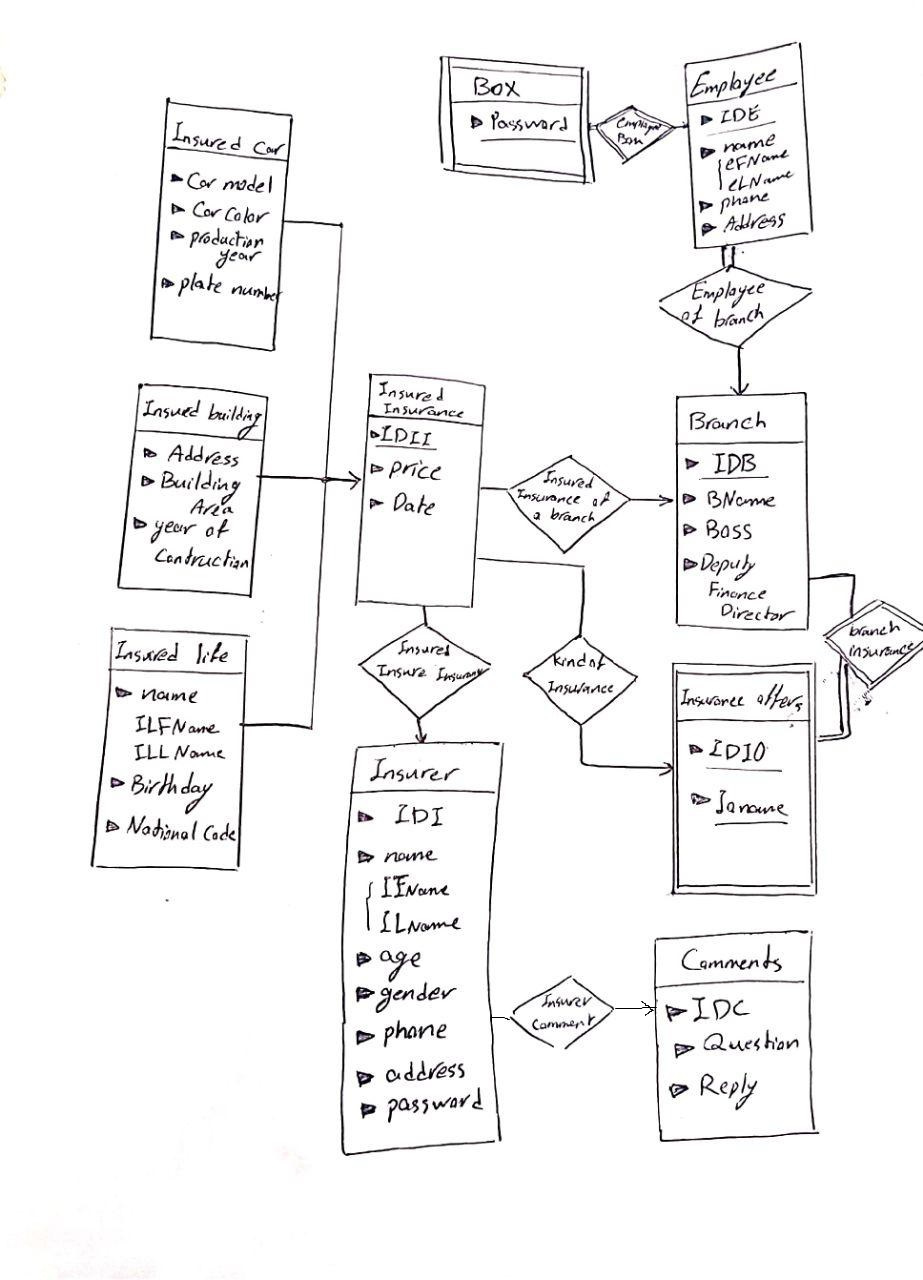
\includegraphics[width = 0.49\linewidth]{chart}
%\caption{محیط نوشته شده با php}
\end{center}
\end{figure}
\end{question}








\section{github}\label{chpt2}
تمامی فایل های تمرینات این درس در آدرس زیر در 
\href{https://github.com/mohammadraziei/DB2019/}{github}
قابل دسترسی می باشد.

\begin{latin}
\begin{center}
\href{https://github.com/MohammadRaziei/DB2019/tree/master/Workspace/HWs}{https://github.com/MohammadRaziei/DB2019/tree/master/Workspace/HWs}
\end{center}
\end{latin}



\begin{center}
\vspace{1.5cm}
\huge
پایان
\end{center}
\end{document}